\documentclass[alsotrans]{beamerswitch}
\usepackage{sdp}

\title{Дървета за търсене}

\date{12--16 декември 2019 г.}

\titlegraphicx{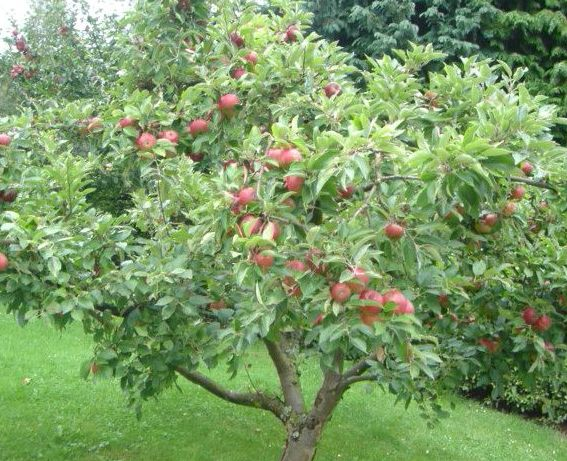
\includegraphics[height=0.25\textheight]{images/searchtree.jpg}\\
  \imageAttr{Appletree}{User:MKFF}{https://commons.wikimedia.org/wiki/File:Appletree_2.jpg}{CC0}}

\forestset{
  % стил по подразбиране за дървета
  default/.style={
    baseline,
    for tree={
      fill=diagramblue,
      draw,circle,
      inner sep=0pt,
      minimum size=3.5ex,
      edge=->}},
  % схематични дървета, с по-големи възли
  scheme/.style={
    default,
    for tree={minimum size=6ex}},
  % поддърво
  tri/.style={
    shape=isosceles triangle,
    shape border rotate=90,
    minimum height=12ex,
    child anchor=north,
    anchor=north},
  % малко поддърво
  trismall/.style={
    tri,
    minimum height=8ex},
  % задраскване на възел
  remove/.style={
    tikz={
      \draw[thick,red] (!.north west) -- (!.south east);
      \draw[thick,red] (!.north east) -- (!.south west);}},
  % задраскване на малък възел
  removesmall/.style={
    tikz={
      \draw[thick,red] (!.north west)++(1.5ex,1.5ex) -- ++(3ex,-3ex);
      \draw[thick,red] (!.north west)++(4.5ex,1.5ex) -- ++(-3ex,-3ex);
      \node at (!.north west) [xshift=3ex,circle,draw,inner sep=0.2ex]{Y};}},
}

% примерно двоично дърво
\newcommand{\samplebinordtree}{%
  \begin{forest}
    default [5 [3 [2 [1] [,phantom]] [4]] [8 [6 [,phantom] [7] ] [10]]]
  \end{forest}%
}

\tikzset{bnodemtx/.style={
    basematrix,
    matrix of nodes,
    nodes={
      fill=diagramblue,
      draw,
      inner sep=0pt,
      align=center,
      minimum height=3.5ex,
      text height=2.5ex,
      text depth=.5ex,
    },
    inner sep=0pt,
  }
}     

\newcommand{\bnode}[5][]{
  \matrix[bnodemtx,nodes={text width=1.6em},#1]
  (#2data) { #3 \& #4 \& #5\\ };
  \matrix[bnodemtx,nodes={text width=1.2em},below=-2*\pgflinewidth of #2data.south]
  (#2next) { \&\&\& \\};
}

\begin{document}

\begin{frame}
  \titlepage
\end{frame}

\begin{frame}
  \frametitle{Дървета за търсене}
  \begin{itemize}
  \item Организация, която позволява бързо намиране на елементи в дървото
  \item Разчита на \textbf{линейна наредба} на елементите
  \item Основни операции:
    \begin{itemize}
    \item \tt{create()} --- създаване на празно дърво за търсене
    \item \tt{insert(x)} --- включване на елемент
    \item \tt{remove(x)} --- изключване на елемент
    \item \tt{search(x)} --- търсене на елемент
    \end{itemize}
  \item Обикновено елементите са двойки (ключ, стойност)
  \item Елементите са наредени относно ключовете си
  \item Стойностите носят данните на елемента
  \end{itemize}
\end{frame}

\section{Двоично дърво за търсене}

\begin{frame}
  \frametitle{Двоично дърво за търсене}
  \begin{definition}[Двоично дърво за търсене]
    \begin{itemize}
    \item Празното дърво $\bot$ е ДДТ
    \item $(X,L,R)$ е ДДТ, ако
      \begin{itemize}
      \item $X$ е по-голямо от от всички елементи в $L$
      \item $X$ е по-малко от от всички елементи в $R$
      \item $L$ и $R$ също са ДДТ
      \end{itemize}
    \end{itemize}
  \end{definition}
  \pause
  \textbf{Пример:}
  \vspace{-2ex}
  \begin{center}
    \small
    \samplebinordtree
  \end{center}
\end{frame}

\begin{frame}
  \frametitle{Търсене на елемент}
  \begin{center}
    \begin{forest}
      scheme [{=X} [<X,tri] [>X,tri]]
    \end{forest}
  \end{center}
\end{frame}

\begin{frame}
  \frametitle{Включване на елемент}
  \small
  \begin{columns}[t,onlytextwidth]
    \begin{column}{0.3\textwidth}
      \begin{forest}
        scheme
        [X [Y<X,anchor=north] [,tri]]
      \end{forest}
    \end{column}
    \pause
    \begin{column}{0.3\textwidth}
      \begin{forest}
        scheme
        [X [,tri] [Y>X,anchor=north]]
      \end{forest}
    \end{column}
    \pause
    \begin{column}{0.4\textwidth}
      \begin{forest}
        scheme
        [X [<X,tri] [>X,tri]]
        \node at (!1.center) [yshift=3.5ex,xshift=-0.4ex,inner sep=0.2ex,draw,circle]{Y};
        \node at (!2.center) [yshift=4.1ex,xshift=0.8ex,inner sep=0.2ex,draw,circle]{Y};
      \end{forest}
    \end{column}
  \end{columns}
\end{frame}

\begin{frame}
  \frametitle{Изключване на елемент}
  \small
  \begin{columns}[t,onlytextwidth]
    \begin{column}{0.3\textwidth}
      \begin{forest}
        scheme
        [\textbf{Y},remove [,tri,phantom] [,tri]]
      \end{forest}
    \end{column}
    \pause
    \begin{column}{0.3\textwidth}
      \begin{forest}
        scheme
        [\textbf{Y},remove [,tri] [,tri,phantom]]
      \end{forest}
    \end{column}
    \pause
    \begin{column}{0.4\textwidth}
      \begin{forest}
        scheme
        [X [<X,tri,removesmall] [>X,tri,removesmall]]
      \end{forest}
    \end{column}
  \end{columns}
\end{frame}

\begin{frame}
  \frametitle{Изключване на елемент --- общ случай}
  \small
  \begin{columns}[t,onlytextwidth]
    \begin{column}{0.5\textwidth}
      \begin{forest}
        scheme
        [\textbf{Y},remove [<Y<M,tri] [>M,tri,parent anchor=south west [M [,trismall,phantom] [>M\\<M',align=center,trismall]] [,tri,phantom]]]
      \end{forest}
    \end{column}
    \pause
    \begin{column}{0.5\textwidth}
      \begin{forest}
        scheme
        [M [<M,tri] [>M,tri,parent anchor=south west [>M\\<M',align=center,trismall] [,trismall,phantom]]]
      \end{forest}
    \end{column}
  \end{columns}
\end{frame}

\section{Балансирани дървета}

\begin{frame}
  \frametitle{Оптимална височина на дърво}
  Сложността на всички операции за двоично дърво до търсене е $O(h)$, където $h$ е височината на дървото.\\[2ex]
  Знаем, че $\log_2 (n+1) \leq h \leq n$.
  \begin{itemize}
  \item $h = n \leftrightarrow $ дървото е изродено до списък
  \item $h = \log_2(n+1)$, когато дървото е пълно
  \item \alert{само тогава ли?}
  \end{itemize}
\end{frame}

\begin{frame}
  \frametitle{Балансирано дърво}
  \begin{definition}[Балансирано дърво]
    \begin{itemize}
    \item Празното дърво $\bot$ е балансирано
    \item $(X,L,R)$ е балансирано, ако
      \begin{itemize}
      \item $|h(L) - h(R)| \leq 1$
      \item<alert@2> $L$ и $R$ също са балансирани
      \end{itemize}
    \end{itemize}
  \end{definition}
  \pause
  \small
  \begin{columns}[t]
    \begin{column}{0.5\textwidth}
      \begin{center}
        \begin{forest}
          default [1 [2 [3 [4] [,phantom]] [,phantom]] [5 [,phantom]
          [6]]]
        \end{forest}
      \end{center}
    \end{column}
    \pause
    \begin{column}{0.5\textwidth}
      \begin{center}
        \begin{forest}
          default [1 [2 [3] [4]] [5 [,phantom] [6]]]
        \end{forest}
      \end{center}
    \end{column}
  \end{columns}
\end{frame}

\begin{frame}
  \frametitle{Оптимална височина на балансирано дърво}
  \begin{theorem}
    За балансирани дървета височината е възможно най-малка\pause, т.е. $h = \lceil log_2 (n+1) \rceil$.
  \end{theorem}
  \pause
  \alert{Обратното вярно ли е?}\\[2ex]
  \pause
  Не!
  \begin{forest}
    default
    [1 [2 [3] [4]] [,phantom]]
  \end{forest}
\end{frame}

\begin{frame}
  \frametitle{Идеално балансирано дърво}
  \begin{definition}[Идеално балансирано дърво]
    \begin{itemize}
    \item Празното дърво $\bot$ е идеално балансирано
    \item $(X,L,R)$ е идеално балансирано, ако
      \begin{itemize}
      \item $|s(L) - s(R)| \leq 1$, където $s(T)$ означава броя на възлите в $T$
      \item $L$ и $R$ също са идеално балансирани
      \end{itemize}
    \end{itemize}
  \end{definition}
  \pause
  \textbf{Пример:}
  \begin{center}
    \begin{forest}
      default [1 [2 [3] [4]] [5 [,phantom] [6]]]
    \end{forest}
  \end{center}
\end{frame}

\begin{frame}
  \frametitle{Балансирани и идеално балансирани дървета}
  Каква е връзката между балансирани и идеално балансирани дървета?
  \pause
  \begin{theorem}
    Всяко идеално балансирано дърво е балансирано.
  \end{theorem}
  \pause
  \begin{proof}
    Индукция по височината на дървото.
  \end{proof}
  \pause
  \alert{Обратното вярно ли е?}
  \pause
  Не:
  \begin{forest}
    default [1 [2 [3] [4]] [5]]
  \end{forest}
\end{frame}

\begin{frame}
  \frametitle{Построяване на идеално балансирано дърво}
  По даден сортиран списък можем да построим идеално балансирано двоично дърво за търсене.\\[2ex]
  Строим рекурсивно:
  \begin{itemize}
  \item Избираме за корен $X$ ``средния'' елемент на списъка
  \item Лявото поддърво строим от подсписъка вляво от ``средния'' елемент
  \item Дясното поддърво строим от подсписъка вдясно от ``средния'' елемент
  \item Двата подсписъка имат приблизително равни дължини
  \item Рекурсията ни гарантира идеална балансираност
  \end{itemize}
  \begin{center}
    \makecommand{\m}{\cellcolor{red!60}}
    \makecommand{\l}{\cellcolor{green!60}}
    \makecommand{\r}{\cellcolor{blue!60}}
    \begin{tabular}{*{12}{|c}|}
      \hline
      \l1&\l2&\l3&\l4&\l5&\l6&\m7&\r8&\r9&\r10&\r11&\r12\\
      \hline
    \end{tabular}
  \end{center}
\end{frame}

\section{AVL дървета}

\begin{frame}
  \frametitle{Самобалансиращи се дървета за търсене}
  Можем да постигнем сложност $O(\log n)$ на операциите търсене, включване и изключване, ако работим само с балансирани дървета.\\[2ex]
  \pause
  \textbf{Идея:} ако дървото се разбалансира след включване или изключване, да го балансираме наново.\\[2ex]
  \pause
  Има различни вариации на самобалансиращи се дървета:
  \begin{itemize}
  \item 2-3 дърво
  \item<alert@4> AVL дърво
  \item червено-черно дърво
  \item косо дърво (splay tree)
  \item Декартово дърво (treap)
  \end{itemize}
  \pause
\end{frame}

\begin{frame}
  \frametitle{AVL дърво}
  Предложено от Адельсон-Велский и Ландис през 1962 г.\\[2ex]
  \textbf{Основна идея:} Всяко поддърво $T = (X,L,R)$ поддържа коефициент на баланс:
  \begin{equation*}
    b(T) = h(R) - h(L)
  \end{equation*}
  \pause
  \begin{block}{}
    \begin{center}
      Едно AVL дърво $T$ е балансирано\\
      $\Longleftrightarrow$\\
      $b(T') \in \{-1,0,1\}$ за всяко поддърво $T'$ на $T$
    \end{center}
  \end{block}
\end{frame}

\begin{frame}
  \frametitle{Самобалансиране}
  \begin{itemize}[<+->]
  \item Операциите за включване и изключване може да променят баланса на някой възел!
  \item Промяната няма как да е с повече от $\pm 1$ (защо?)
  \item Разбалансиране се получава при $b(T) = \pm 2$
    \begin{itemize}
    \item $b(T) = -2$ --- лявото поддърво е с 2 нива по-високо от дясното
      \begin{itemize}
      \item<7-> ``завъртаме надясно'' за да балансираме
      \end{itemize}
    \item $b(T) = 2$ --- дясното поддърво е с 2 нива по-високо от лявото
      \begin{itemize}
      \item<8-> ``завъртаме наляво'' за да балансираме
      \end{itemize}
    \end{itemize}
  \item
    Дефинираме операции за ``завъртане'', които възстановяват баланса.
  \end{itemize}
\end{frame}

\begin{frame}[label=rotright]
  \frametitle{Завъртане надясно (zig)}
  \begin{center}
    \small
    \begin{forest}
      default [Y [X [A,trismall] [B,trismall]] [C,trismall]]
    \end{forest}
    {\Huge$\curvearrowright$}
    \begin{forest}
      default [X [A,trismall] [Y [B,trismall] [C,trismall]]]
    \end{forest}
  \end{center} \pause \vspace{-2.5ex}
  \begin{overlayarea}{\textwidth}{24ex}
    \onslide<+->
    \begin{onlyenv}<.-.(12)>
      $$ b'(Y) = ? $$
    \end{onlyenv}
    \onslide<+->
    \begin{onlyenv}<.-.(5)>
      \textbf{I сл. }$b(X) \geq 0$
      \onslide<+-> $\Rightarrow h(B) \geq h(A)$
      \onslide<+-> $\Rightarrow h(X) = h(B) + 1$
      \onslide<+-> $\Rightarrow b(Y) = h(C) - h(X)$
      \onslide<+-> $ = \underbrace{h(C) - h(B)}_{b'(Y)} - 1$
      \onslide<+-> $\Rightarrow b'(Y) = b(Y) + 1$
    \end{onlyenv}
    \onslide<+->
    \begin{onlyenv}<.-.(5)>
      \textbf{II сл.} $b(X) < 0$
      \onslide<+-> $\Rightarrow h(B) < h(A)$
      \onslide<+-> $\Rightarrow h(X) = h(A) + 1$
      \onslide<+-> $\Rightarrow b(Y) = h(C) - h(A) - 1$
      \onslide<+-> $ = \underbrace{h(C) - h(B)}_{b'(Y)} + \underbrace{h(B) - h(A)}_{b(X)} - 1$
      \onslide<+-> $\Rightarrow b'(Y) = b(Y) - b(X) + 1$
    \end{onlyenv}
    \onslide<+->
    \begin{onlyenv}<.,.(14)->
      \begin{equation*}
        b'(Y) =
        \begin{cases}
          b(Y) + 1,&\text{ ако }b(X) \geq 0,\\
          b(Y) - b(X) + 1,&\text{ ако }b(X) < 0.
        \end{cases}
      \end{equation*}
    \end{onlyenv}
    \onslide<+->
    \begin{onlyenv}<.-.(12)>
      $$ b'(X) = ? $$
    \end{onlyenv}
    \onslide<+->
    \begin{onlyenv}<.-.(5)>
      \textbf{I сл. }$b'(Y) \leq 0$
      \onslide<+-> $\Rightarrow h(B) \geq h(C)$
      \onslide<+-> $\Rightarrow h'(Y) = h(B) + 1$
      \onslide<+-> $\Rightarrow b'(X) = h'(Y) - h(A)$
      \onslide<+-> $ = \underbrace{h(B) - h(A)}_{b(X)} + 1$
      \onslide<+-> $\Rightarrow b'(X) = b(X) + 1$
    \end{onlyenv}
    \onslide<+->
    \begin{onlyenv}<.-.(5)>
      \textbf{II сл.} $b'(Y) > 0$
      \onslide<+-> $\Rightarrow h(B) < h(C)$
      \onslide<+-> $\Rightarrow h'(Y) = h(C) + 1$
      \onslide<+-> $\Rightarrow b'(X) = h(C) + 1 - h(A)$
      \onslide<+-> $ = \underbrace{h(C) - h(B)}_{b'(Y)} + \underbrace{h(B) - h(A)}_{b(X)} + 1$
      \onslide<+-> $\Rightarrow b'(X) = b(X) + b'(Y) + 1$
    \end{onlyenv}
    \onslide<+->
    \begin{onlyenv}<.->
      \begin{equation*}
        b'(X) =
        \begin{cases}
          b(X) + 1,&\text{ ако }b'(Y) \leq 0,\\
          b(X) + b'(Y) + 1,&\text{ ако }b'(Y) > 0.
        \end{cases}
      \end{equation*}
    \end{onlyenv}
    \onslide<+->
    \begin{onlyenv}<.>
      \vspace{-2ex}
      \begin{equation*}
        b'(X) > b(X), \quad b'(Y) > b(Y)
      \end{equation*}
    \end{onlyenv}
  \end{overlayarea}
\end{frame}

\begin{frame}<-5>
  \frametitle{Завъртане наляво (zag)}
  \begin{center}
    \small
    \begin{forest}
      default [X [A,trismall] [Y [B,trismall] [C,trismall]]]
    \end{forest}
    {\Huge$\curvearrowleft$}
    \begin{forest}
      default [Y [X [A,trismall] [B,trismall]] [C,trismall]]
    \end{forest}
  \end{center}
  \pause
  \temporal<3>{
    \alert{
      \begin{equation*}
        b'(Y) =
        \begin{cases}
          b(Y) + 1,&\text{ ако }b(X) \geq 0,\\
          b(Y) - b(X) + 1,&\text{ ако }b(X) < 0.
        \end{cases}
      \end{equation*}
      \begin{equation*}
        b'(X) =
        \begin{cases}
          b(X) + 1,&\text{ ако }b'(Y) \leq 0,\\
          b(X) + b'(Y) + 1,&\text{ ако }b'(Y) > 0.
        \end{cases}
      \end{equation*}
    }
  }
  {
    \alert{
      \begin{equation*}
        b(Y) =
        \begin{cases}
          b'(Y) + 1,&\text{ ако }b'(X) \geq 0,\\
          b'(Y) - b'(X) + 1,&\text{ ако }b'(X) < 0.
        \end{cases}
      \end{equation*}
      \begin{equation*}
        b(X) =
        \begin{cases}
          b'(X) + 1,&\text{ ако }b(Y) \leq 0,\\
          b'(X) + b(Y) + 1,&\text{ ако }b(Y) > 0.
        \end{cases}
      \end{equation*}
    }
  }
  {
    \begin{equation*}
      b'(Y) =
      \begin{cases}
        b(Y) - 1,&\text{ ако }b'(X) \geq 0,\\
        b(Y) + b'(X) - 1,&\text{ ако }b'(X) < 0.
      \end{cases}
    \end{equation*}
    \begin{equation*}
      b'(X) =
      \begin{cases}
        b(X) - 1,&\text{ ако }b(Y) \leq 0,\\
        b(X) - b(Y) - 1,&\text{ ако }b(Y) > 0.
      \end{cases}
    \end{equation*}
  }
  \onslide<5>
  \begin{equation*}
    b'(X) < b(X), \quad b'(Y) < b(Y)
  \end{equation*}
\end{frame}

\begin{frame}[label=balright]
  \frametitle{Балансиране надясно}
  \begin{center}
    \scriptsize
    \begin{forest}
      default [Z [Y [X [A,trismall] [B,trismall]] [C,trismall]] [D,trismall]]
    \end{forest}
    {\Huge$\curvearrowright$}
    \begin{forest}
      default [Y [X [A,trismall] [B,trismall]] [Z [C,trismall] [D,trismall]]]
    \end{forest}
  \end{center}
  \begin{itemize}[<+->]
  \item Въртим надясно, ако $b(Z) = -2$
  \item \alert{Внимание:} Ако $b(Y) = 1$, то
    \begin{itemize}
    \item $b'(Z) = b(Z) + 1  = -1$
    \item $b'(Y) = b(Y) + 1 = \alert2$
    \end{itemize}
  \item Трябва да подсигурим, че $b(Y) \leq 0$...
  \item ...с предварително завъртане наляво!
  \end{itemize}
\end{frame}

\begin{frame}
  \frametitle{Двойно балансиране надясно (zag-zig)}
  \begin{center}
    \tiny
    \begin{forest}
      default [Z [X [A,trismall] [Y [B,trismall] [C,trismall]]] [D,trismall]]
    \end{forest}
    {\LARGE$\curvearrowleft$}
    \begin{forest}
      default [Z [Y [X [A,trismall] [B,trismall]] [C,trismall]] [D,trismall]]
    \end{forest}
    {\LARGE$\curvearrowright$}
    \begin{forest}
      default [Y [X [A,trismall] [B,trismall]] [Z [C,trismall] [D,trismall]]]
    \end{forest}
  \end{center}
  \begin{itemize}[<+->]
  \item Ако $b(X) = 1$, първо завъртаме наляво около $X$.
  \item Така $b'(X) \leq 0$ и $b'(Y) \leq 0$
  \item Вече можем да завъртим надясно около $Y$.
  \item След балансиране сме сигурни, че $h'(Y) < h(Z)$, т.е. намаляваме височината.
  \end{itemize}
\end{frame}

\begin{frame}
  \frametitle{Балансиране наляво}
  \begin{center}
    \scriptsize
    \begin{forest}
      default [X [A,trismall] [Y [B,trismall] [Z [C,trismall] [D,trismall]]]]
    \end{forest}
    {\Huge$\curvearrowleft$}
    \begin{forest}
      default [Y [X [A,trismall] [B,trismall]] [Z [C,trismall] [D,trismall]]]
    \end{forest}
  \end{center}
  \begin{itemize}[<+->]
  \item Въртим наляво, ако $b(Z) = 2$
  \item \alert{Внимание:} Ако $b(Y) = -1$, то
    \begin{itemize}
    \item $b'(Z) = b(Z) - 1  = 1$
    \item $b'(Y) = b(Y) - 1 = \alert{-2}$
    \end{itemize}
  \item Трябва да подсигурим, че $b(Y) \geq 0$...
  \item ...с предварително завъртане надясно!
  \end{itemize}
\end{frame}

\begin{frame}
  \frametitle{Двойно балансиране наляво (zig-zag)}
  \begin{center}
    \tiny
    \begin{forest}
      default [X [A,trismall] [Z [Y [B,trismall] [C,trismall]] [D,trismall]]]
    \end{forest}
    {\LARGE$\curvearrowright$}
    \begin{forest}
      default [X [A,trismall] [Y [B,trismall] [Z [C,trismall] [D,trismall]]]]
    \end{forest}
    {\LARGE$\curvearrowleft$}
    \begin{forest}
      default [Y [X [A,trismall] [B,trismall]] [Z [C,trismall] [D,trismall]]]
    \end{forest}
  \end{center}
  \begin{itemize}[<+->]
  \item Ако $b(Z) = -1$, първо завъртаме надясно около $Z$.
  \item Така $b'(Z) \geq 0$ и $b'(Y) \geq 0$
  \item Вече можем да завъртим наляво около $Y$.
  \item След балансиране сме сигурни, че $h'(Y) < h(X)$, т.е. намаляваме височината.
  \end{itemize}
\end{frame}

\begin{frame}
  \frametitle{Кога да балансираме?}
  \begin{itemize}[<+->]
  \item Когато включваме или изключваме елемент, трябва да следим кога балансът се променя
  \item При промяна на баланс ще трябва да пребалансираме
  \item Затова ще реализираме включването и изключването \textbf{рекурсивно}
  \item На обратния ход на рекурсията ще пребалансираме при нужда
  \item Балансът се променя когато височината на детето се е увеличила или намалила
  \end{itemize}
\end{frame}

\begin{frame}
  \frametitle{Балансиране при включване и изключване}
  Балансиране при включване
  \onslide<+->
  \begin{itemize}[<+->]
  \item При дъното на \textbf{включването} височината винаги се увеличава с 1
  \item Ако височината на \textbf{по-ниското дете} се увеличи, то височината на родителя не се променя
  \item При балансиране винаги компенсираме за увеличената височина на детето
  \end{itemize}
  \onslide<+->
  Балансиране при изключване
  \begin{itemize}[<+->]
  \item При дъното на \textbf{изключването} дъното височината винаги се намалява с 1
  \item Ако височината на \textbf{по-високото дете} се намали, то височината на родителя не се променя
  \item Ако след балансиране $b(T) \neq 0$, значи сме компенсирали за намалената височина на детето
  \item Ако след балансиране $b(T) = 0$, значи височината се е намалила
  \end{itemize}
\end{frame}

\section{B-дървета}

\begin{frame}
  \frametitle{B-дървета}
  \begin{definition}[B-дърво]
    B-дърво от ред $n$ наричаме $n$-арно дърво ($n \geq 3$), за което:
    \begin{itemize}
    \item всички листа са на еднаква височина
    \item всеки възел съдържа най-много $n-1$ ключа подредени в нарастващ ред
    \item всеки възел (освен корена) съдържа най-малко $\left\lfloor\frac {n-1}2\right\rfloor$ ключа
    \item всеки възел с $m$ ключа $k_1,\ldots,k_m$ или няма поддървета, или има точно $m+1$ непразни поддървета $T_0,\ldots, T_m$, които са разположени максимално вляво (т.е. $T_{m+1},\ldots,T_n$ са празни).
    \item $k_i$ е по-голям от всички ключове в поддърветата $T_j$ за $j \leq i$
    \item $k_i$ е по-малък от всички ключове в поддърветата $T_j$ за $j > i$
    \end{itemize}
  \end{definition}
\end{frame}

\begin{frame}
  \frametitle{Пример за B дърво от ред 4}
  \begin{center}
    \ttfamily
    \begin{tikzpicture}
      \bnode{b1}38-
      \bnode[below left =of b1next]{b2}12-
      \bnode[below      =of b1next]{b3}4--
      \bnode[below right=of b1next]{b4}{10}{12}{15}

      \draw[pointer] (b1next-1-1.center) to (b2data);
      \draw[pointer] (b1next-1-2.center) to (b3data);
      \draw[pointer] (b1next-1-3.center) to (b4data);
      \nullptr{b1next-1-4}
      \foreach \node in {2,3,4} {
        \foreach \idx in {1,2,3,4} {
          \nullptr{b\node next-1-\idx}
        }}
    \end{tikzpicture}
  \end{center}
\end{frame}

\begin{frame}
  \frametitle{Включване на елемент}
  % TODO: да се анимират различните случаи с TikZ
  \begin{itemize}[<+->]
  \item Прави се опит за включване на елемент в някое листо
  \item Ако се окаже, че се опитваме да включим елемент в листо, което вече е пълно с $n-1$ ключа:
    \begin{itemize}
    \item Разцепваме възела на два други с приблизително еднакъв брой елементи
    \item Средния по големина ключ се опитваме да вмъкнем в родителя
    \item Ако в родителя вече има $n-1$ ключа, повтаряме същата схема
    \item Ако стигнем до корена, правим нов корен само с един ключ и две поддървета
    \end{itemize}
  \end{itemize}
\end{frame}

\begin{frame}
  \frametitle{Изключване на елемент}
  % TODO: да се анимират различните случаи с TikZ
  \begin{itemize}[<+->]
  \item Първо намираме ключа $K$ на елемента в дървото
    \begin{itemize}
    \item Ако е в листо, изтриваме го
    \item Ако е във вътрешен възел, заменяме го с:
      \begin{itemize}
      \item най-малкия ключ $>K$, или
      \item най-големия ключ $<K$
      \item такъв ключ задължително ще се намира в листо
      \end{itemize}
    \end{itemize}
  \item Ако броят на ключовете в листото падне под минимума:
    \begin{itemize}
    \item Опитваме се да заемем ключ и съответно поддърво от някой от двата съседа
    \item Ако и двата съседа също съдържат минимален брой ключове
      \begin{itemize}
      \item Листото се слива с някой от двата си съседа
      \item Понеже броят на поддърветата в родителя намалява с 1, прехвърляме в листото ключа, който е стоял между двете слети листа в родителя
      \item Сигурни сме, че в новото листо броят ключове не надвишава максимума, понеже $2\left\lfloor\frac{n-1}2\right\rfloor \leq n - 1$
      \end{itemize}
    \end{itemize}
    \item Ако сега броят на ключовете в родителя падне под минимума, повтаряме същата процедура за него
  \end{itemize}
\end{frame}

\end{document}
